\subsection*{Section 1.3}
\textbf{Problem 2}

For $\der{y}{x} = 2x+y$,
\begin{enumerate}
    \item Find and sketch the solution through $(0,-2)$
    \item Sketch the solution through $(-1,3)$
    \item What can you say about the solution 
        as $x \to \infty$ and $x \to -\infty$?
\end{enumerate}

\solution
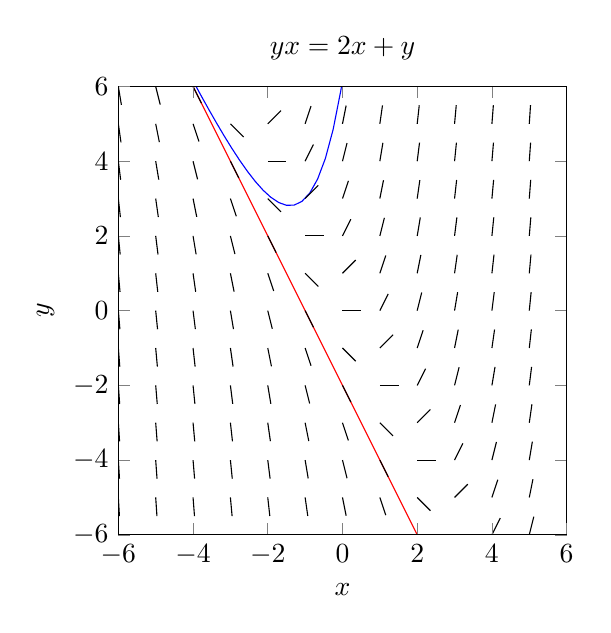
\begin{tikzpicture}
    \begin{axis}[
        xmin = -6, xmax = 6,
        ymin = -6, ymax = 6,
        zmin = 0, zmax = 1,
        axis equal image,
        view = {0}{90},
        title = {$\der{y}{x} = 2x+y$},
        xlabel = {$x$},
        ylabel = {$y$},
    ]
    \addplot[red, domain=-6:6]{-2*x-2};
    \addplot[blue, domain=-4:1]{3*e^(x+1)-2*x-2};
    \addplot3[
        quiver = {
            u = {1/sqrt(1+(2*x+y)^2)},
            v = {(2*x+y)/sqrt(1+(2*x+y)^2)},
            scale arrows = 0.5,
        },
        samples = 13,
        domain = -6:6,
        domain y = -6:6,
    ] {0};
    \end{axis}
\end{tikzpicture}

\begin{enumerate}
    \item The solution through $(0, -2)$ is shown by the red curve.
        The slope is
        \[
            \der{y}{x}|_{x=0} 
            = 2(0) + y 
            = y 
            = -2
        \]
        In order for the point to pass through $(0, -2)$, 
        the y-intercept must be $-2$.
        Therefore, the equation of the line is $y = -2x-2$.
    \item The solution through $(-1, 3)$ is shown by the blue curve.
    \item The solution goes to $\infty$ for both 
        $x \to \infty$ and $x \to -\infty$.
\end{enumerate}

\textbf{Problem 3}

For $\der{v}{t} = 1-\frac{v}{8}$, 
sketch the solutions for $v(0) = 5, 8, 15$
Why is $v=8$ the terminal velocity?

\solution

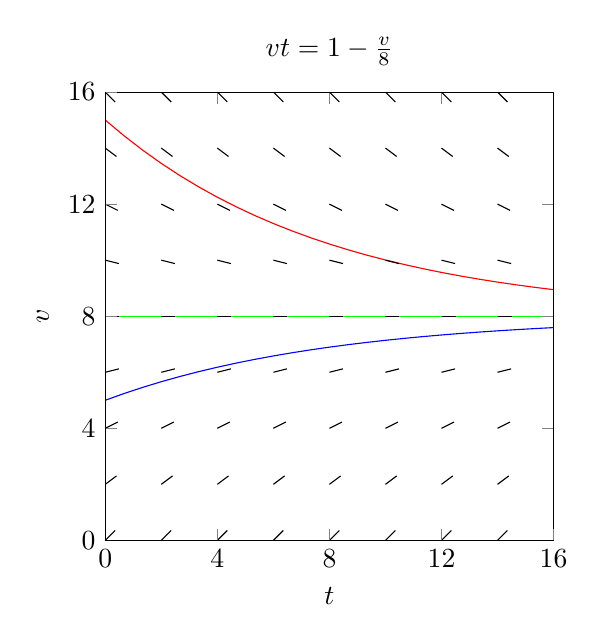
\begin{tikzpicture}
    \begin{axis}[
        xmin = 0, xmax = 16,
        ymin = 0, ymax = 16,
        zmin = 0, zmax = 1,
        axis equal image,
        view = {0}{90},
        title = {$\der{v}{t} = 1-\frac{v}{8}$},
        xlabel = {$t$},
        ylabel = {$v$},
        xtick = {0,4,8,12,16},
        xticklabels = {$0$,$4$,$8$,$12$,$16$},
        ytick = {0,4,8,12,16},
        yticklabels = {$0$,$4$,$8$,$12$,$16$},
    ]
    \addplot[red, domain=0:16]{7*e^(-x/8)+8};
    \addplot[green, domain=0:16]{8};
    \addplot[blue, domain=0:16]{-3*e^(-x/8)+8};
    
    \addplot3[
        quiver = {
            u = {1/sqrt(1+(1-y/8)^2)},
            v = {(1-y/8)/sqrt(1+(1-y/8)^2)},
            scale arrows = 0.5,
        },
        samples = 9,
        domain = 0:16,
        domain y = 0:16,
    ] {0};
    \end{axis}
\end{tikzpicture}

The red curve is the solution for $y(0) = 15$,
the green curve is the solution for $y(0) = 8$,
and the blue curve is the solution for $y(0) = 5$.
8 is the terminal velocity because the velocity approaches 8
for all solutions. \\
\textbf{Problem 6}
Consider 
\[
    \der{y}{x} = x + \sin y
\]
\begin{enumerate}
    \item What is the slope at $(1, \frac{\pi}{2})$?
    \item Argue that the solution curve increases for $x>1$.
    \item Show that all solutions satisfy 
        \[
            \der[2]{y}{x} = 1 + x\cos y + \frac{1}{2} \sin 2y
        \]
    \item Prove that the curve through $(0, 0)$ has a relative minimum at $(0,0)$.
\end{enumerate}
\solution 
\begin{enumerate}
    \item The slope is zero.
    \[
        \der{y}{x} = x + \sin y = 1 + \sin \frac{\pi}{2} = 2
    \]
    \item $\sin y$ can be at minimum $-1$, so 
        $x + \sin y$ must be positive for $x > 1$.
    \item Using the chain rule 
        \begin{align*}
            \der[2]{y}{x} 
            &= 1 + \cos(y) \der{y}{x} \\
            &= 1 + \cos(y)(x + \sin y) \\
            &= 1 + x\cos y + \sin y \cos y \\
            &= 1 + x\cos y + \frac{1}{2} \sin 2y
        \end{align*}
    \item Since $\der{y}{x} = 0$ and $\der[2]{y}{x} = 1 > 0$
        at $(0,0)$, the curve has a relative minimum at this point.
\end{enumerate}
\textbf{Problem 8}
\[
    \der{x}{t} = t^3 - x^3
\]
\begin{enumerate}
    \item What is the velocity at $x=1$ and $t=2$?
    \item Show that the acceleration is
        \[
            \der[2]{x}{t} = 3t^2 - 3t^3x^2 + 3x^5
        \]
    \item Can a particle at $x=2$ and $t=2.5$ 
        reach $x=1$ later?
\end{enumerate}
\solution 
\begin{enumerate}
    \item 
        \[
            \der{x}{t} = 2^3 - 1^3 = 7
        \]
    \item Using implicit differentiation,
        \[
            \der[2]{x}{t} 
            = 3t^2 - 3x^2 \der{x}{t}
            = 3t^2 - 3x^2(t^3 - x^3)
            = 3t^2 -3t^3x^2 - x^5
        \]
    \item Whenever $t > x$, $t^3-x^3 > 0$ so x will increase.
        If $t < x$, x will decrease but only until $t = x$.
        Since the values $t_0$ and $x_0$ are already greater than 1,
        $x$ cannot reach a value of 1 at a later time.
\end{enumerate}
\textbf{Problem 18}

What is the behavior of a solution to the following equation 
as $x \to \infty$?
\[
    \der{y}{x} = -y
\]
\solution

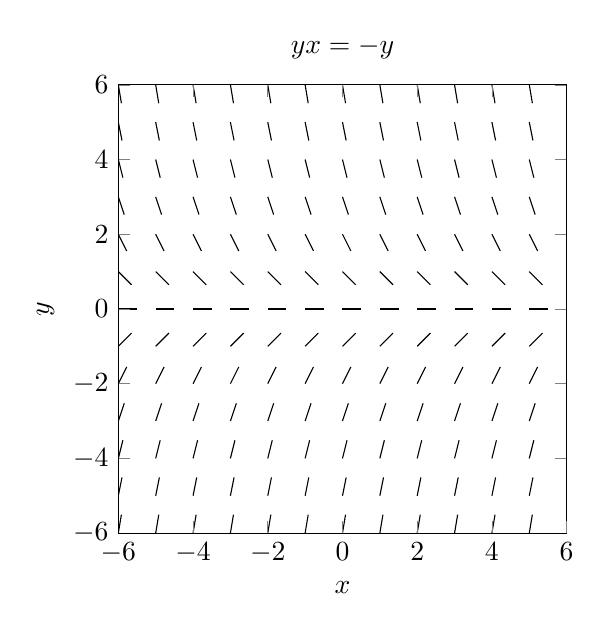
\begin{tikzpicture}
    \begin{axis}[
        xmin = -6, xmax = 6,
        ymin = -6, ymax = 6,
        zmin = 0, zmax = 1,
        axis equal image,
        view = {0}{90},
        title = {$\der{y}{x} = -y$},
        xlabel = {$x$},
        ylabel = {$y$},
    ]
    \addplot3[
        quiver = {
            u = {1/sqrt(1+y^2)},
            v = {-y/sqrt(1+y^2)},
            scale arrows = 0.5,
        },
        samples = 13,
        domain = -6:6,
        domain y = -6:6,
    ] {0};
    \end{axis}
\end{tikzpicture}

$\der{y}{x}$ is negative above the x-axis and positive below it,
so solutions will tend towards $y=0$ as $x \to \infty$.
\newpage